% !TeX root = ../../thesis.tex
\chapter{Applications: Mechanical integrity of infilled structures}\label{ch:infill}

\section{Introduction}

\section{Methods}

\begin{figure}[h]
\centering
\medskip
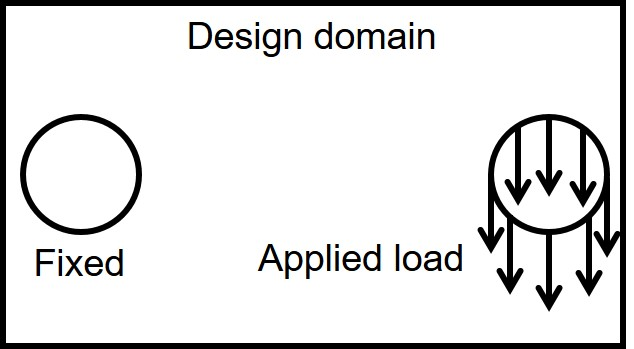
\includegraphics[width=0.5\textwidth]{domain.jpg}
\caption[Computational domain for the topology optimization]{Computational domain for the topology optimization} \label{fig:infill_domain}
\end{figure}


\begin{figure}[h]
\centering
\medskip
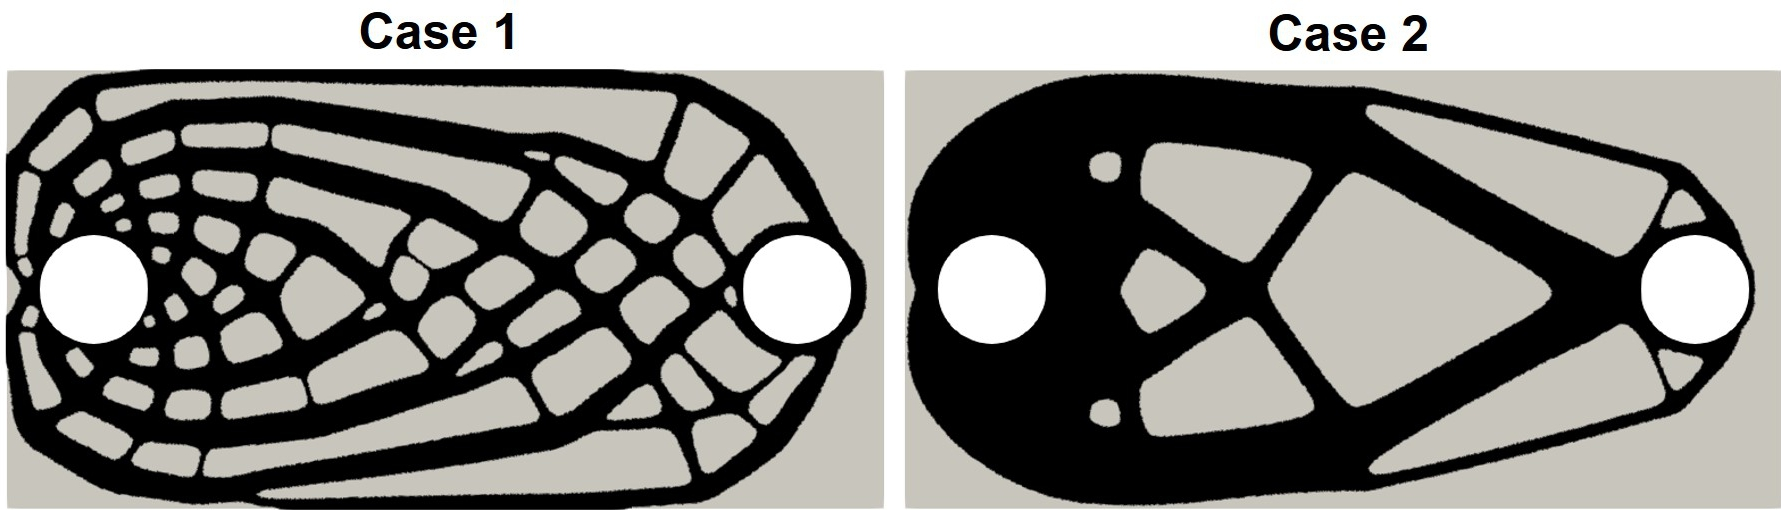
\includegraphics[width=\textwidth]{final_cases.jpg}
\caption[Topology optimization output to be used in the biodegradation simulations]{Topology optimization output to be used in the biodegradation simulations} \label{fig:infill_final_cases}
\end{figure}


\begin{figure}[h]
\centering
\medskip
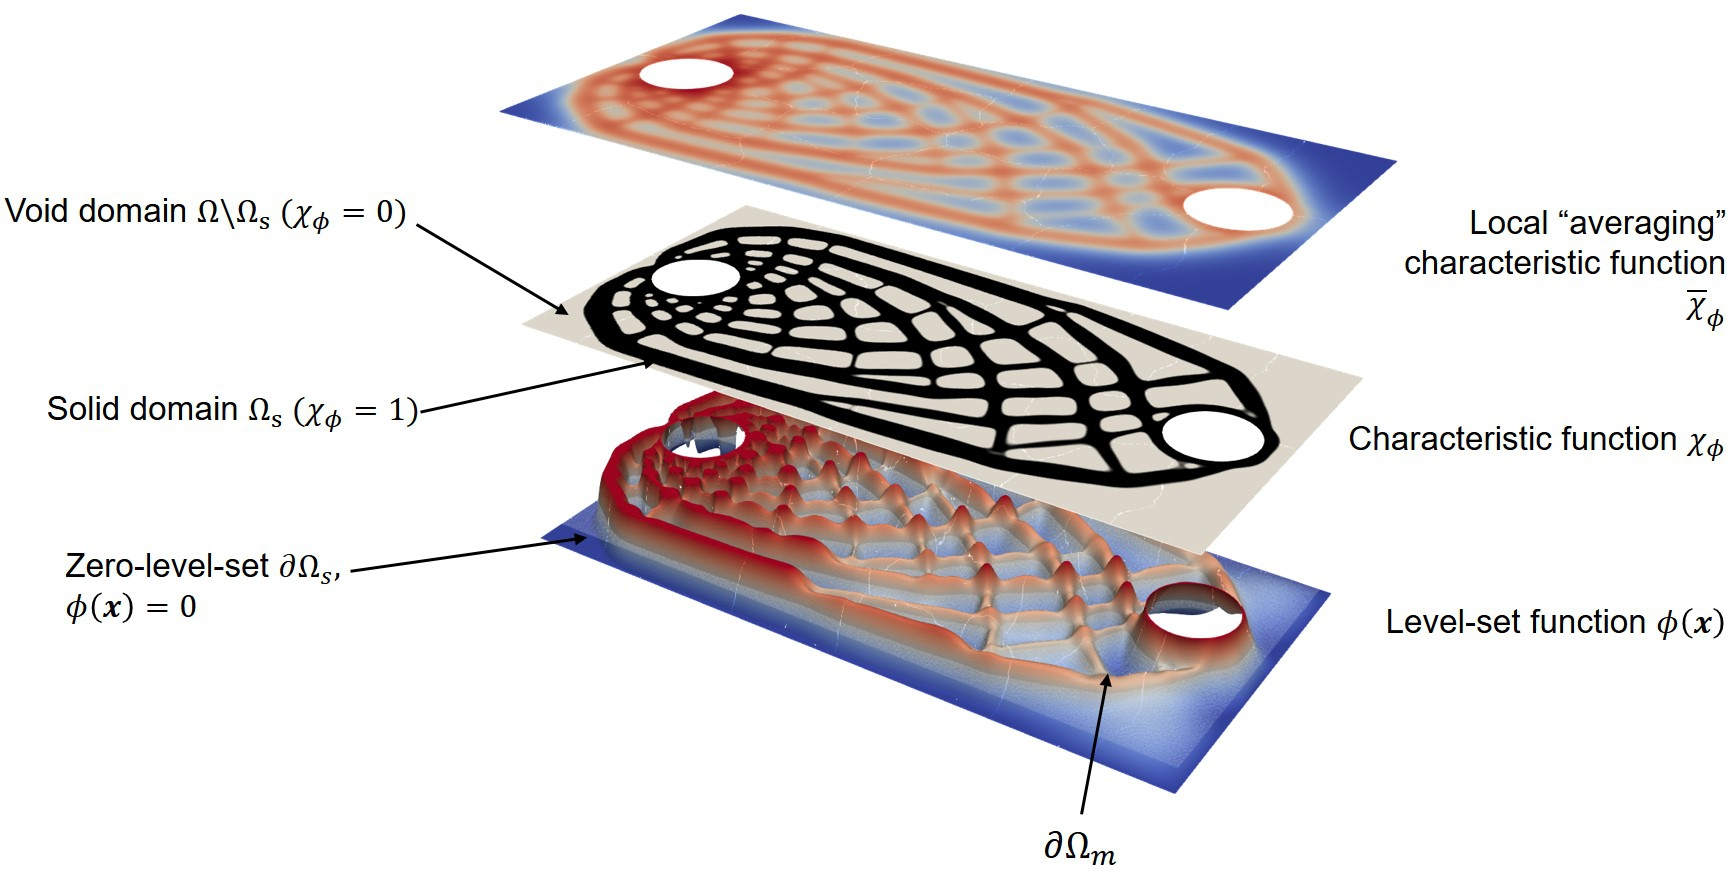
\includegraphics[width=\textwidth]{diagram.jpg}
\caption[Coupling topology optimization and biodegradation models]{Coupling topology optimization and biodegradation models} \label{fig:infill_diagram}
\end{figure}


\begin{figure}[h]
\centering
\medskip
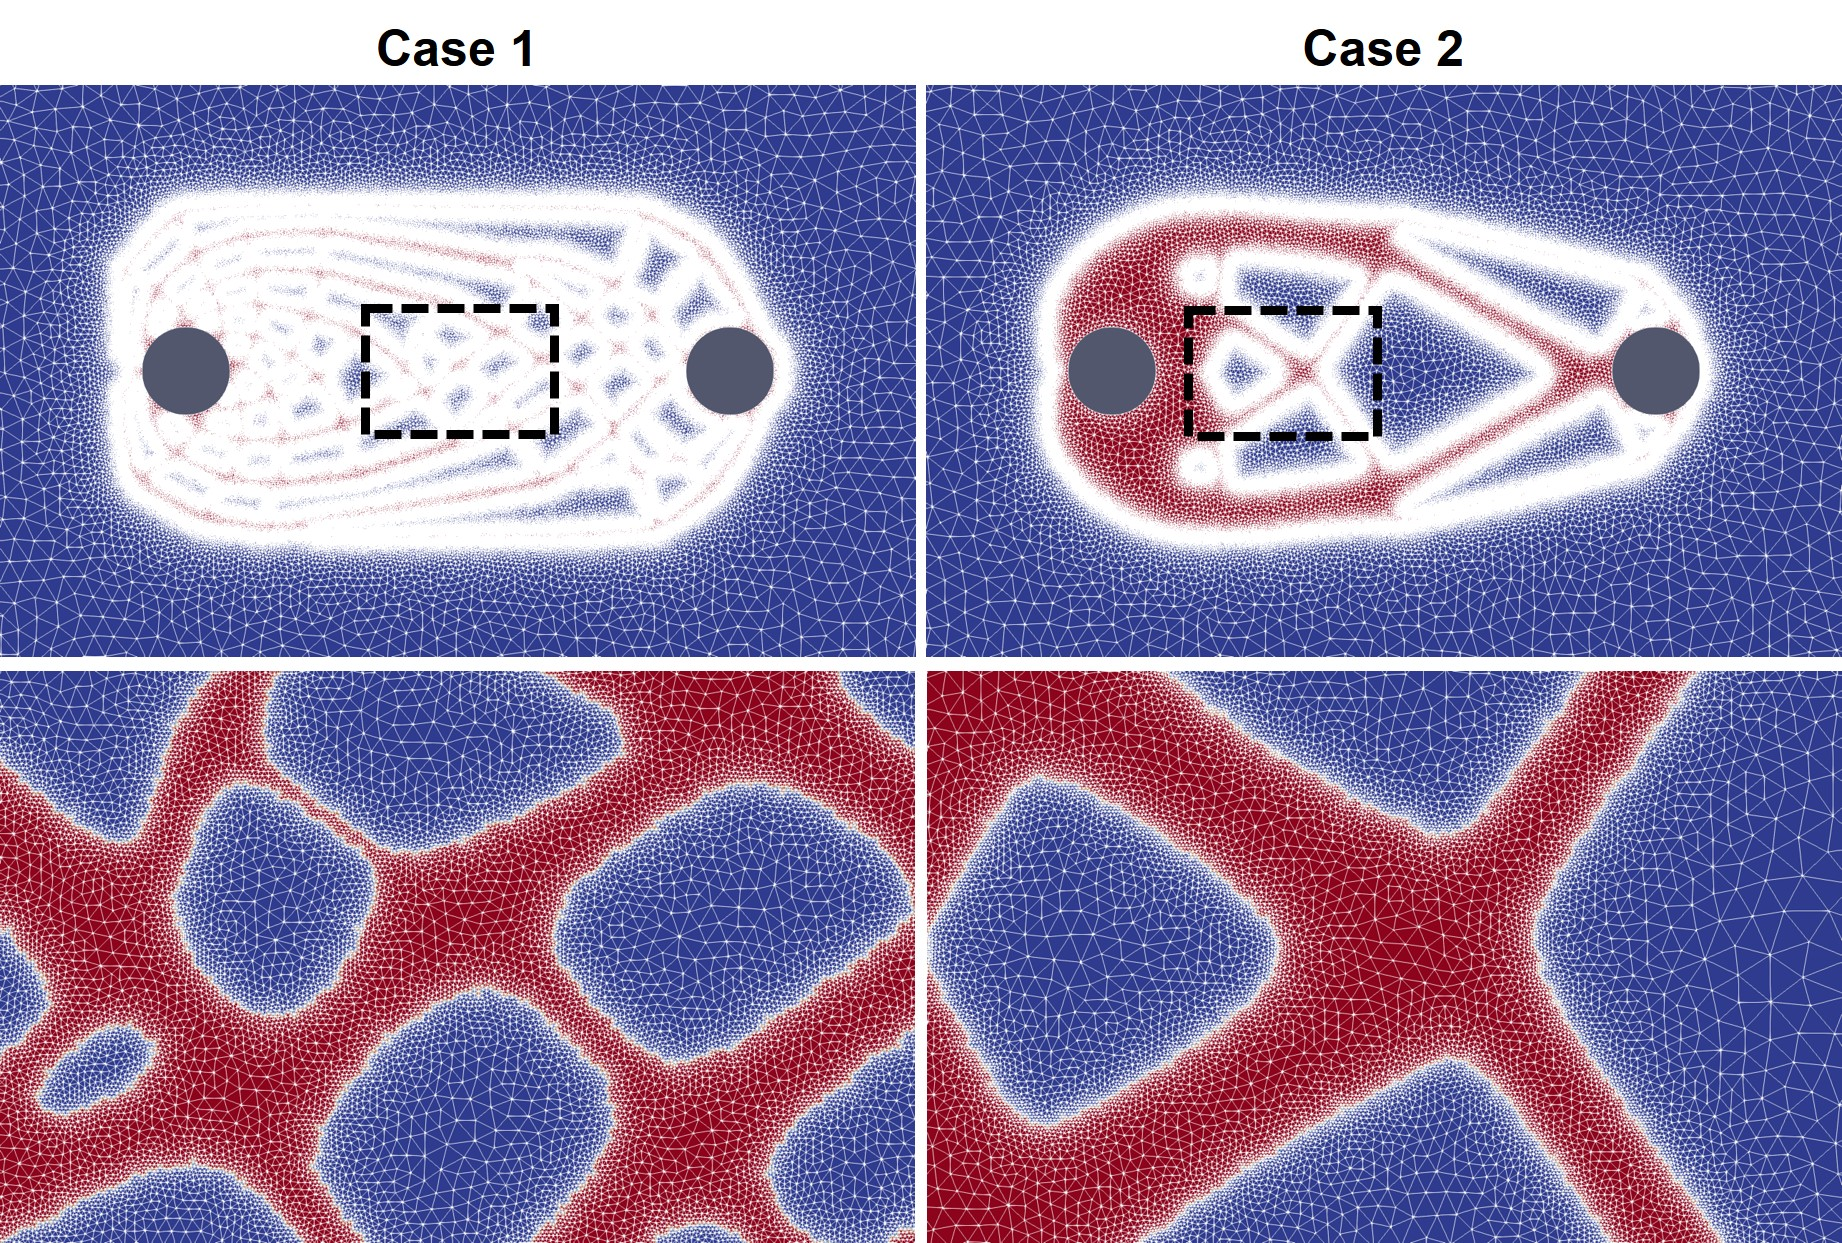
\includegraphics[width=\textwidth]{mesh.jpg}
\caption[Computational mesh for the biodegradation simulations]{Computational mesh for the biodegradation simulations} \label{fig:infill_mesh}
\end{figure}



\section{Results}


\begin{figure}[h]
\centering
\medskip
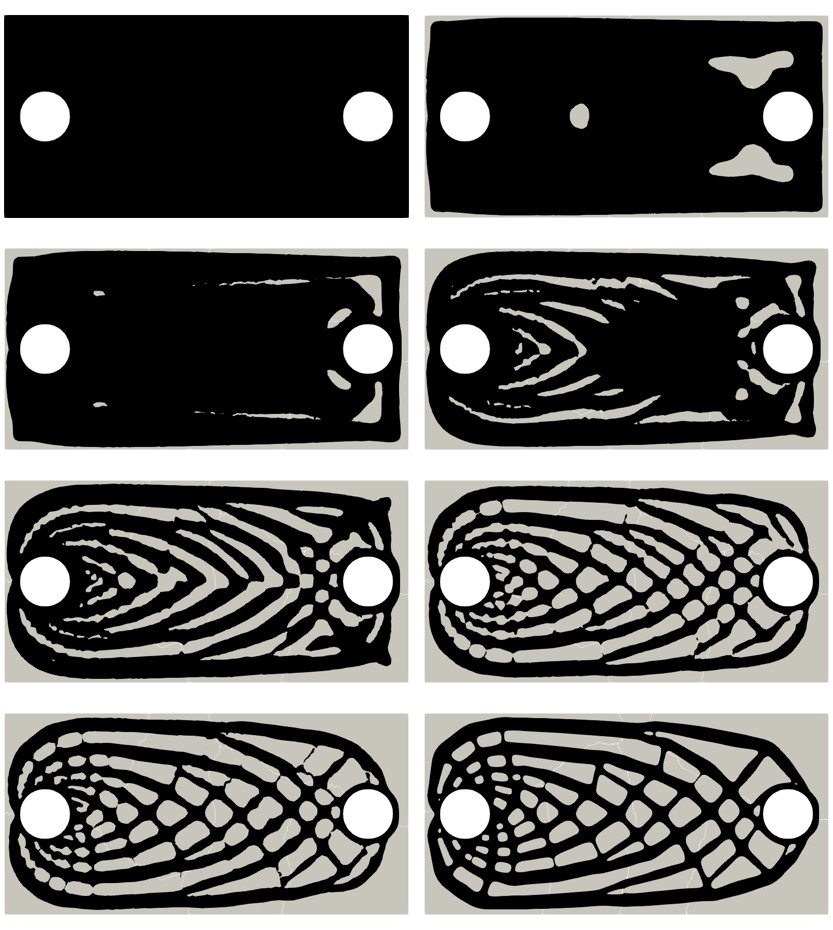
\includegraphics[width=\textwidth]{case1_to_steps.jpg}
\caption[Evolution of the topology optimization level set function for case 1]{Evolution of the topology optimization level set function to get the optimized shape for case 1, in which a local volume constraint was imposed.} \label{fig:infill_case1_to_steps}
\end{figure}

\begin{figure}[h]
\centering
\medskip
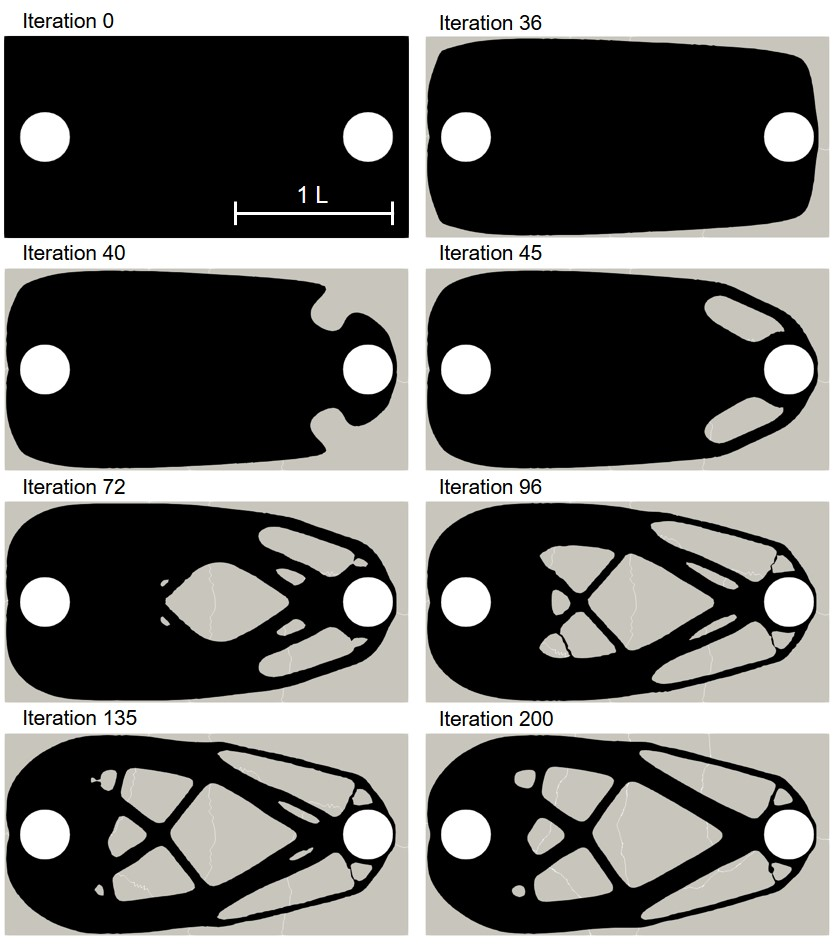
\includegraphics[width=\textwidth]{case2_to_steps.jpg}
\caption[Evolution of the topology optimization level set function for case 2]{Evolution of the topology optimization level set function to get the optimized shape for case 1, where only the global volume constraint was imposed.} \label{fig:infill_case2_to_steps}
\end{figure}



\begin{figure}[h]
\centering
\medskip
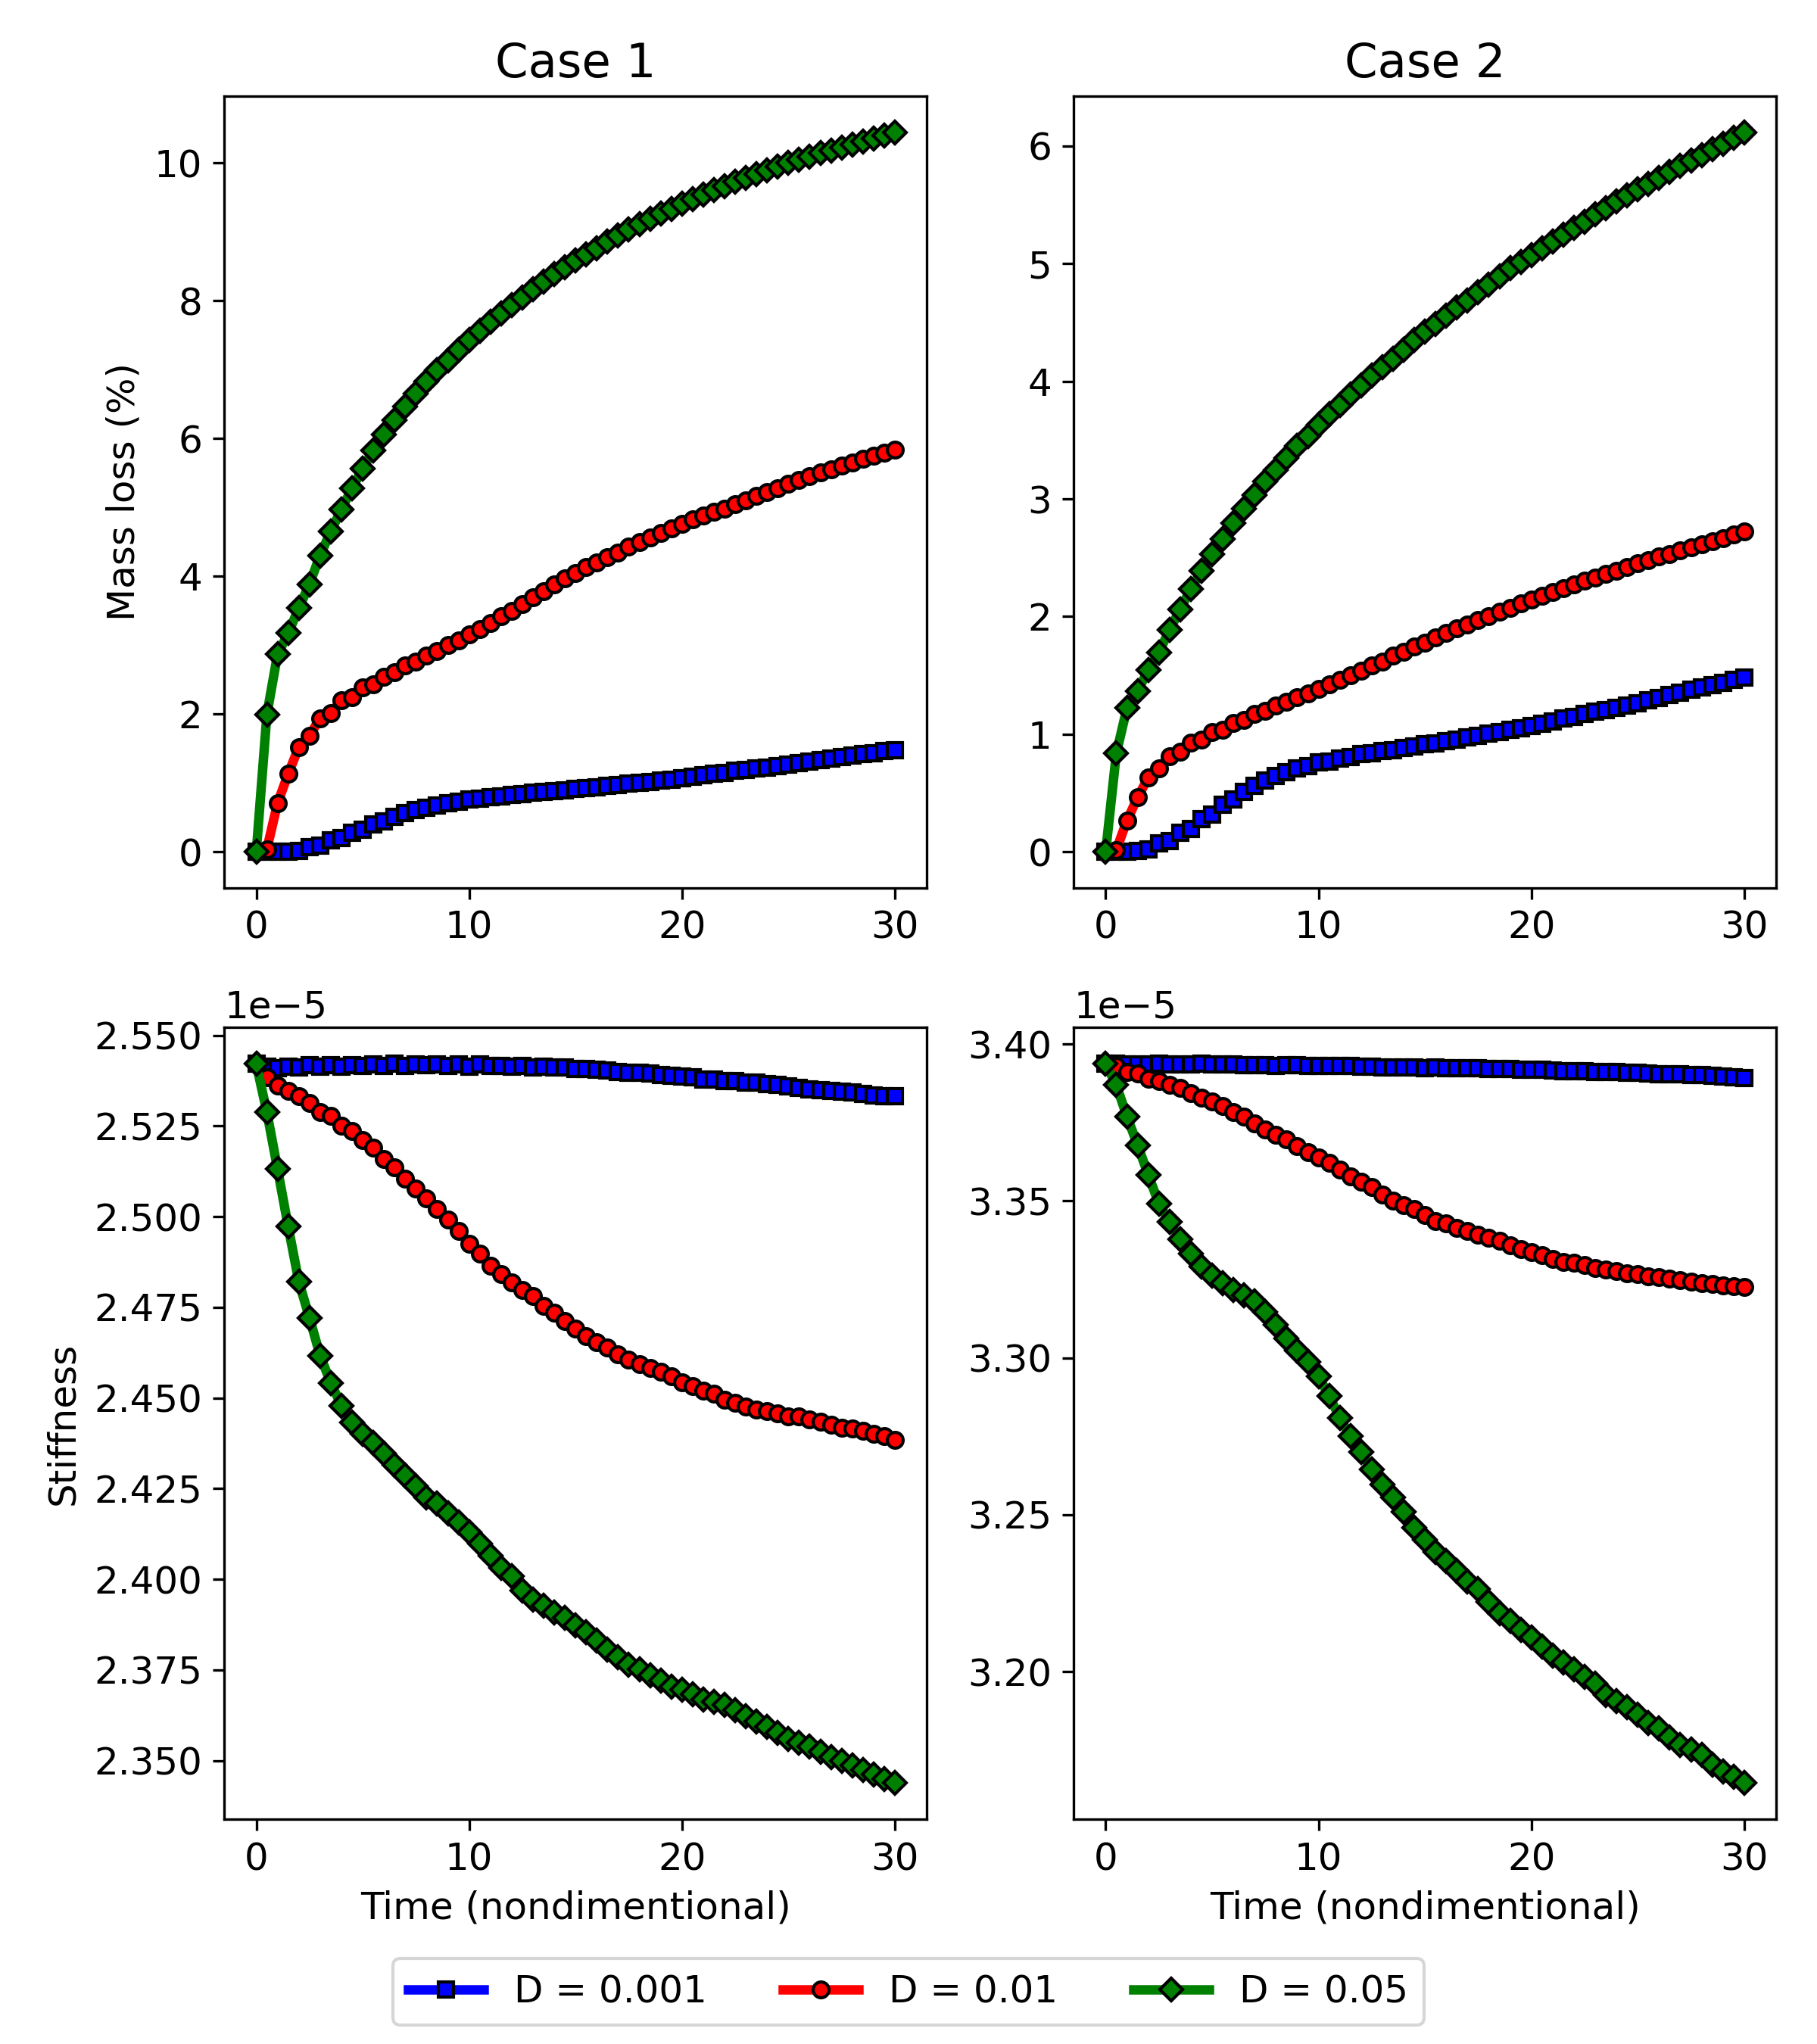
\includegraphics[width=\textwidth]{degradation_stiffness.png}
\caption[Results of the coupled model to predict the stiffness changes during biodegradation]{Results of the coupled model to predict the stiffness changes during biodegradation} \label{fig:infill_degradation_stiffness}
\end{figure}


\begin{figure}[h]
\centering
\medskip
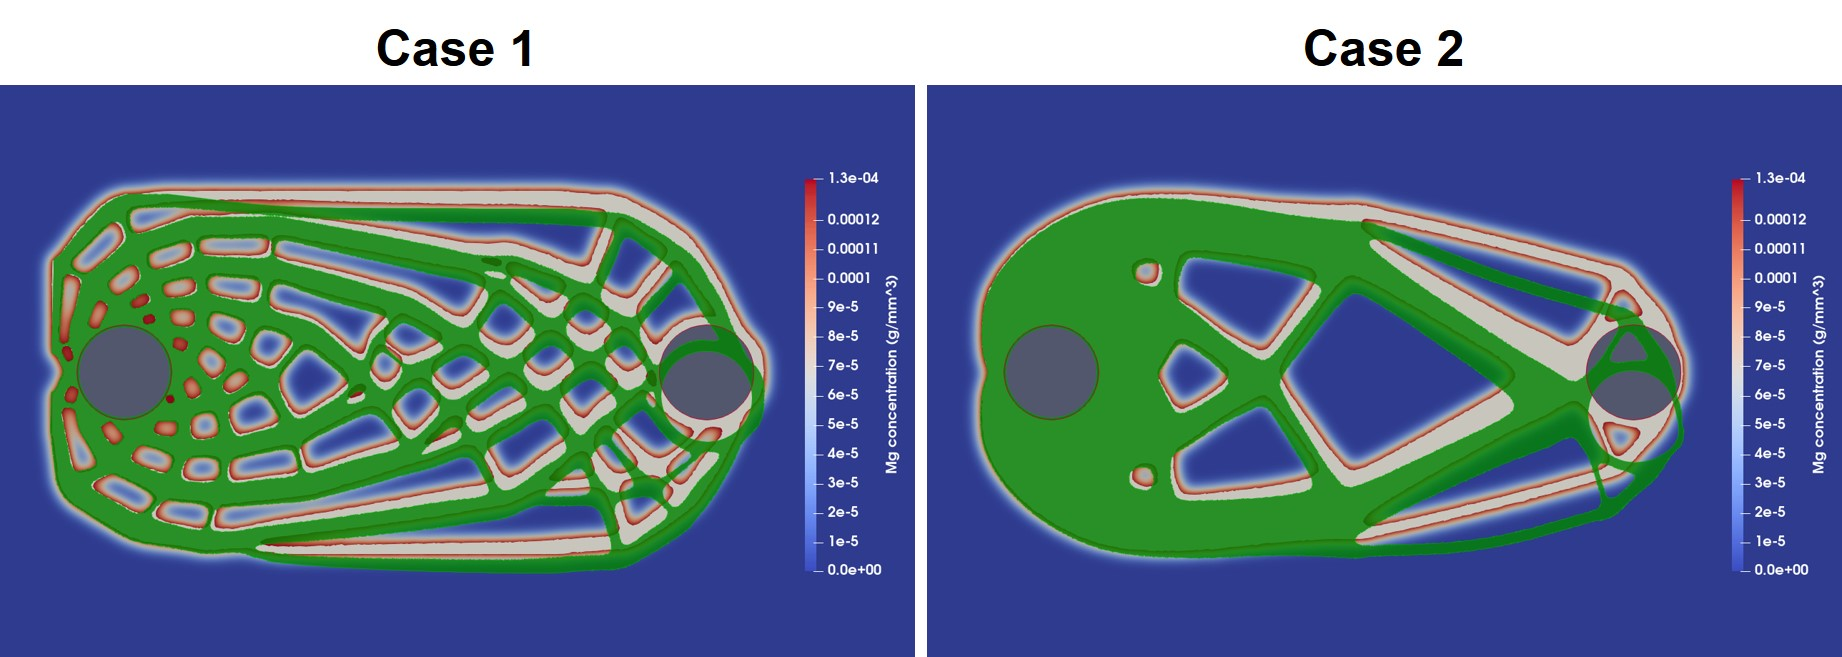
\includegraphics[width=\textwidth]{results_mechanics.jpg}
\caption[Coupled model results showing the stiffness analysis taking place during biodegradation simulation]{Coupled model results showing the stiffness analysis taking place during the biodegradation simulation} \label{fig:infill_results_mechanics}
\end{figure}


\begin{figure}[h]
\centering
\medskip
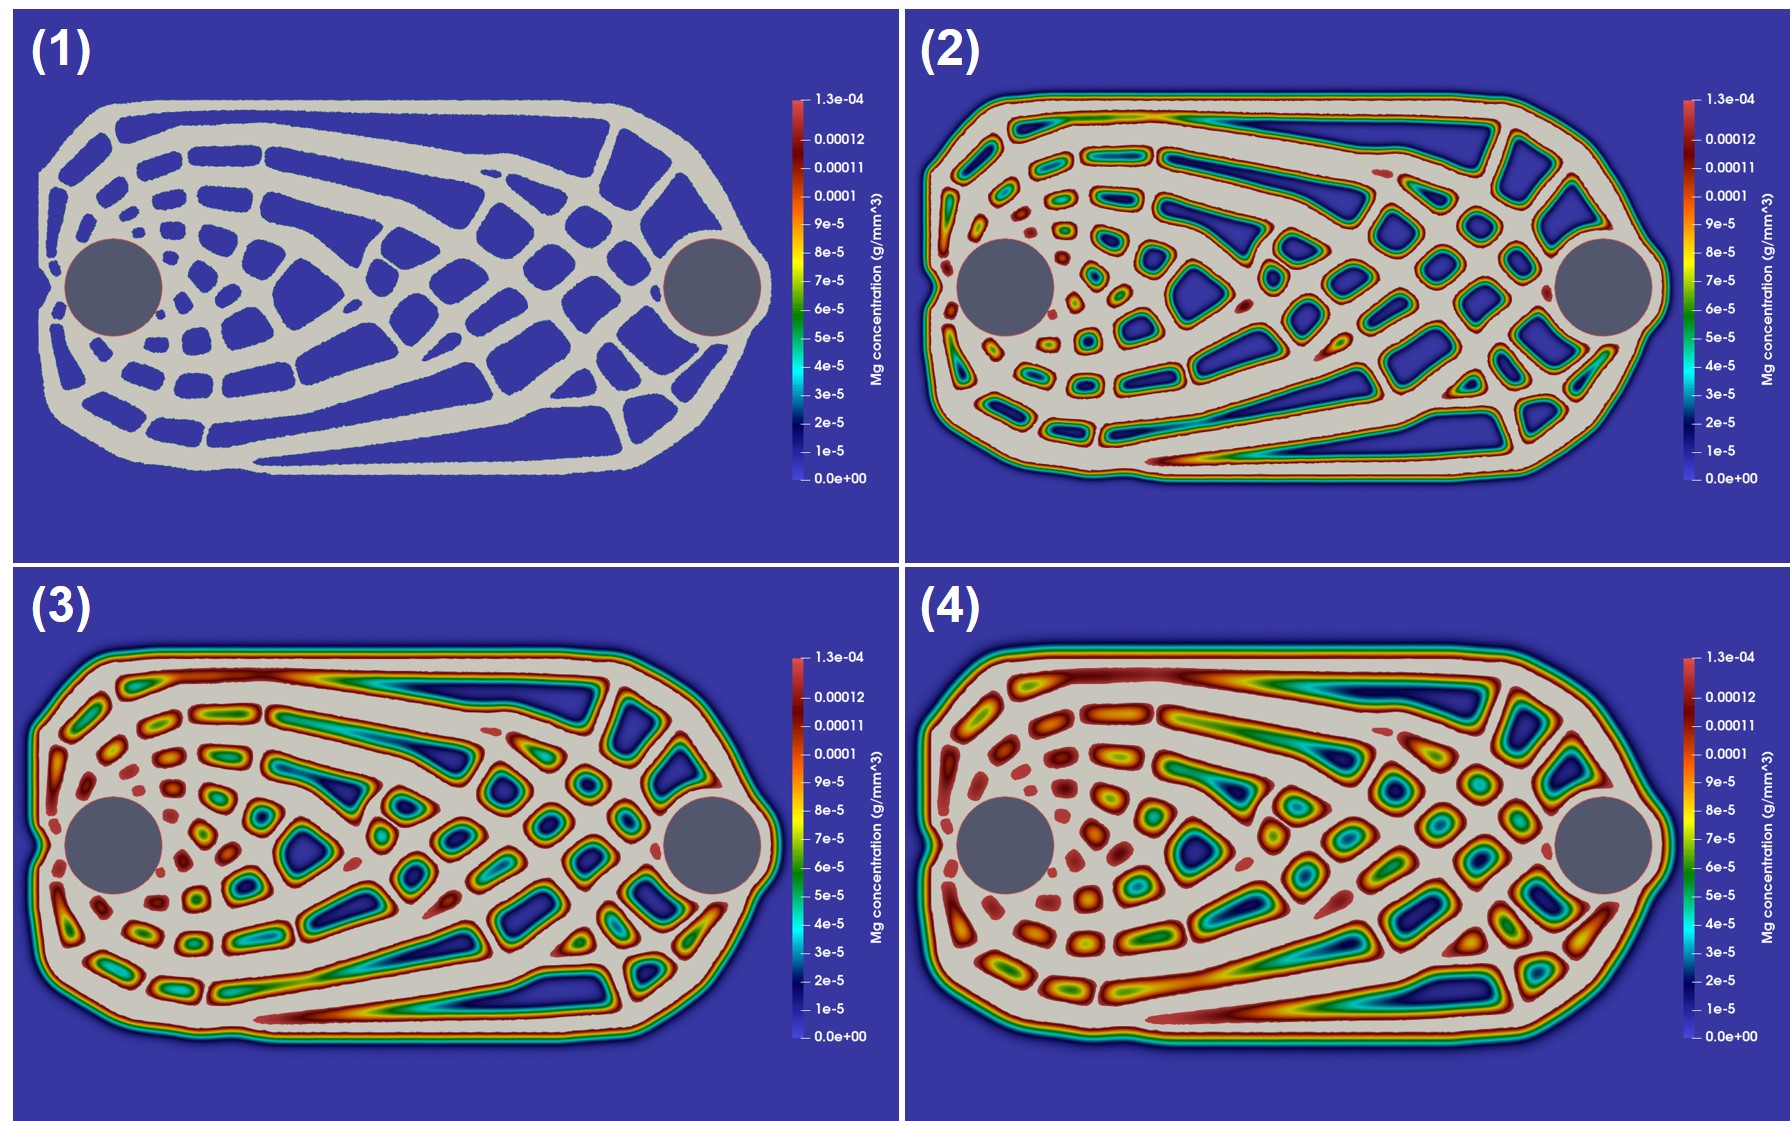
\includegraphics[width=\textwidth]{results_degradation_case1.jpg}
\caption[Visualization of the results of the biodegradation simulation for case 1]{Visualization of the results of the biodegradation simulation for case 1} \label{fig:infill_results_degradation_case1}
\end{figure}


\begin{figure}[h]
\centering
\medskip
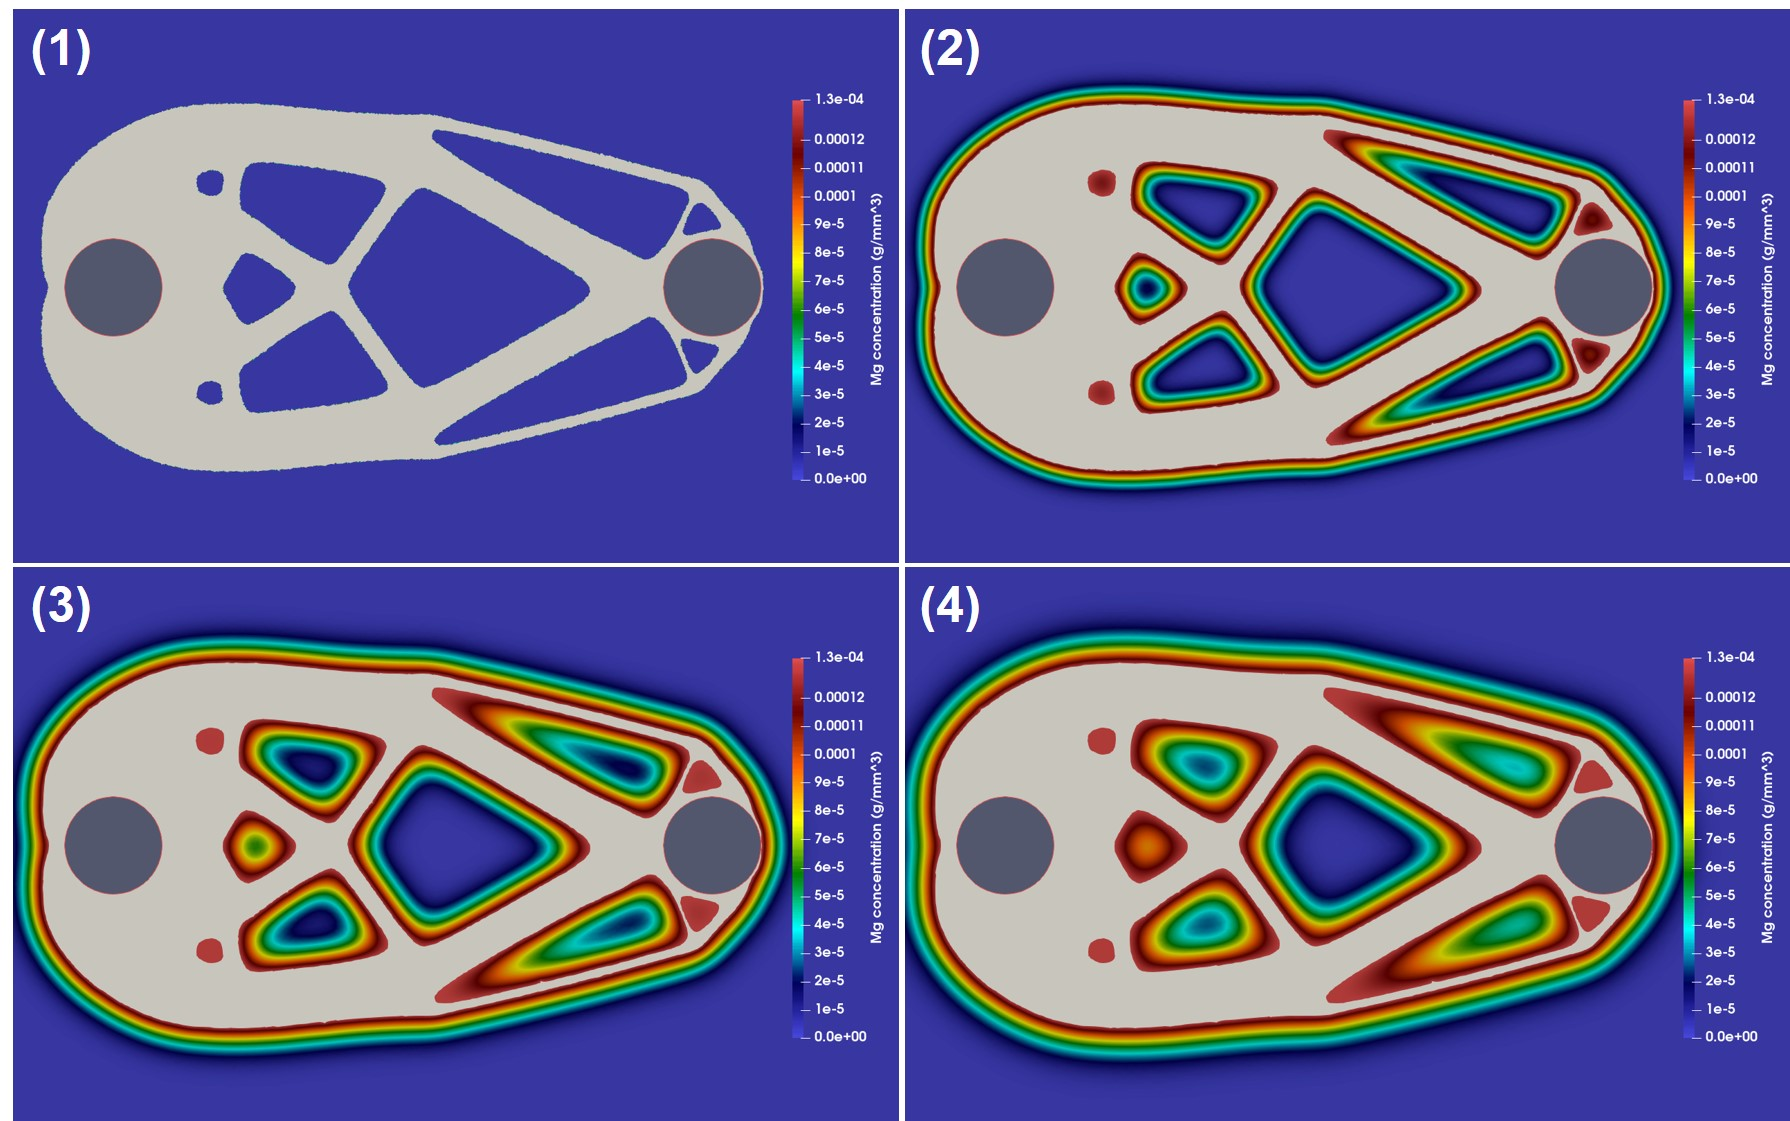
\includegraphics[width=\textwidth]{results_degradation_case2.jpg}
\caption[Visualization of the results of the biodegradation simulation for case 2]{Visualization of the results of the biodegradation simulation for case 2} \label{fig:infill_results_degradation_case2}
\end{figure}


\begin{figure}[h]
\centering
\medskip
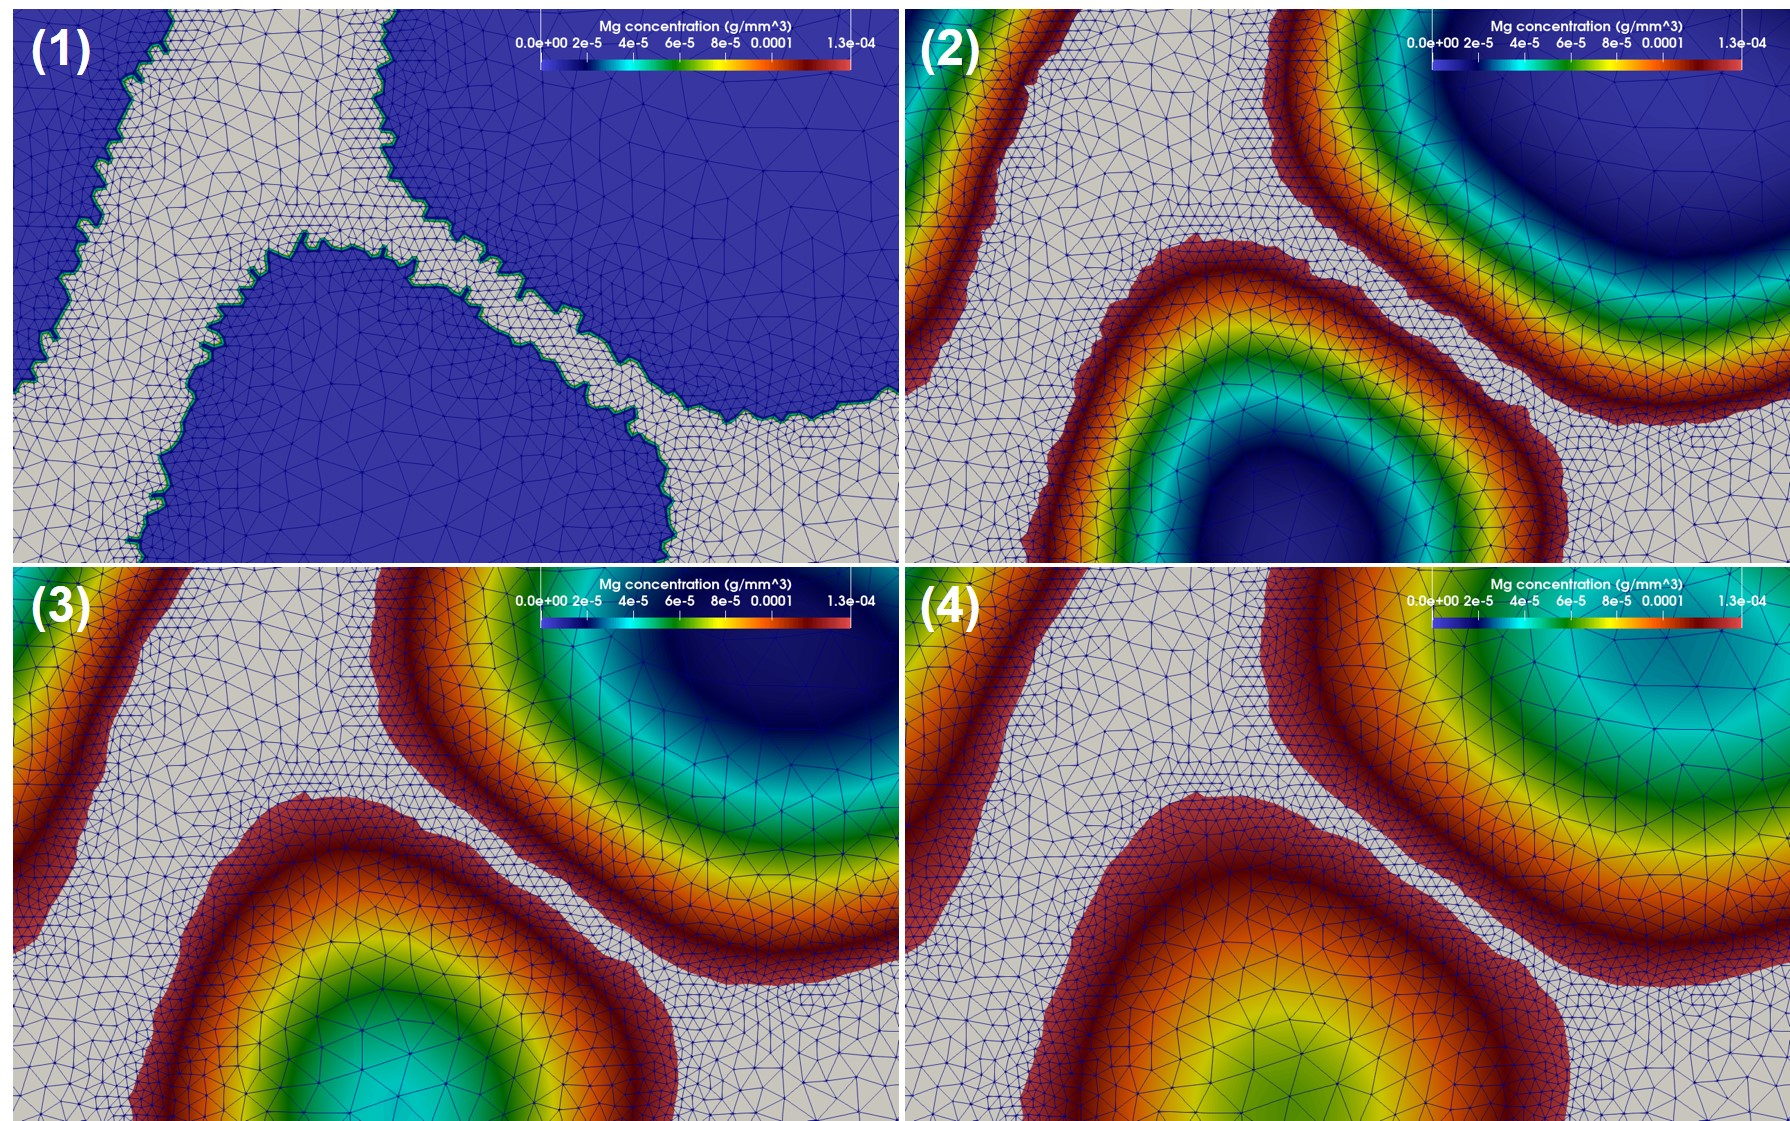
\includegraphics[width=\textwidth]{results_degradation_case1_zoom.jpg}
\caption[Zoom view of the results of the biodegradation simulation for case 1]{Visualization of the results of the biodegradation simulation for case 1, zoomed view} \label{fig:infill_results_degradation_case1_zoom}
\end{figure}

\section{Discussion}


%%%%%%%%%%%%%%%%%%%%%%%%%%%%%%%%%%%%%%%%%%%%%%%%%%
% Keep the following \cleardoublepage at the end of this file, 
% otherwise \includeonly includes empty pages.
\cleardoublepage

